\chapter{Concept and Design}
\label{cha:conceptanddesign}

We need to describe here what do we want to achieve, what do we mean by modelling and visualizing macroscopic movements etc - thus general architecture that we have 3 components, Stop Detection from telekom data based on movements and updates of "areas" in your mobile phone, Clustering of Stops to find most popular "stops" in the city, Graph Generation to find where do the people move and in what amount

\section{Stop Detection}

Analyzing different approaches for stop detection based on localization data (ref. \autoref{cha:introduction_appr_stopdet}), we decided to base our solution on standard human behavior regarding mobility within the cities (ref. \autoref{cha:introduction_hummob}) and reusing the concept of Mobility Index (ref. \autoref{cha:introduction_mob_index_sect})).
\\
\\
Stop detection is divided into two phases:
\begin{description}
	\item[Identifying stop candidates] according to stop detection algorithm
	\item[Reconciliation of stop candidates] taking into account mobility indexes of points. 
\end{description}

\subsection{Identifying stop candidates}

Stop algorithm, shown on \autoref{fig:cd_algorithm}, is considering 3 parameters - MinWalkSpeed, MinTransportSpeed, ThresholdDistance. 
\\\\
So called ThresholdDistance is distance mentioned in \autoref{cha:introduction_dataanaly} (which in case of Berlin been in range 800-1500m) as distances between points, where there is significant "jump" in frequency of occurences, which might mean that at these intervals, continuous points been gathered, and distances over that values might be discontinuous. Furthermore, these distances are relatively small compared to other observed distances, allowing more accurate decision process. We assume, that at these distances, no significant "interuption" in gatharing the points has been introduced in the form of buildings, metro or other factors.
\\\\
Thus, for these higher accuracy points one could assume, that if mobile device have been moving within the minimum walking speed MinWalkSpeed (ref. \autoref{cha:introduction_hummob}), this point is identified as stop candidate. 
\\\\
Thus, for lower accuracy points one could assume, that if mobile device have been moving within the minimum transport speed MinTransportSpeed (ref. \autoref{cha:introduction_hummob}), this point is as well identified as stop candidate. In this example, it could mean, that over longer distance, one could move with transportation with significant speed, stop for longer period and then use fast transportation again, resulting in higher then minimum walking speed, but with speed which is in average lower then other psychological value as minimum transport speed or maximum walking speed.

\begin{figure}[!ht]
	\centering
	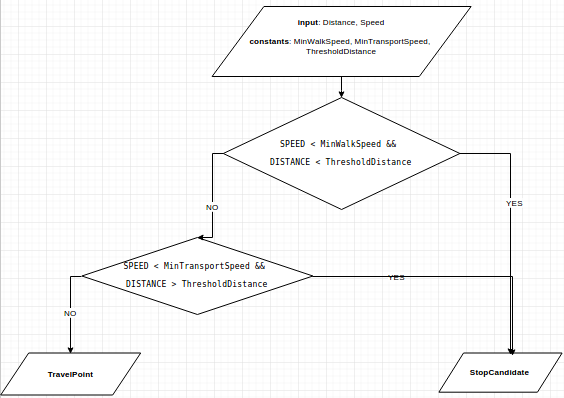
\includegraphics[width=0.8\textwidth]{images/stop_algorithm_1.png}\\
	\caption{First phase of stop detection algorithm  }
	\label{fig:cd_algorithm}
\end{figure}

\subsection{Reconciliation of stop candidates}

\autoref{fig:reco_general} shows that there are many scenarios in which stop candidate has been detected, taking into account movement speed between points, distance and mobility index. In the above example, the mobility index windows was considering past 60 minutes from each of the points. 

\begin{figure}[!ht]
	\centering
	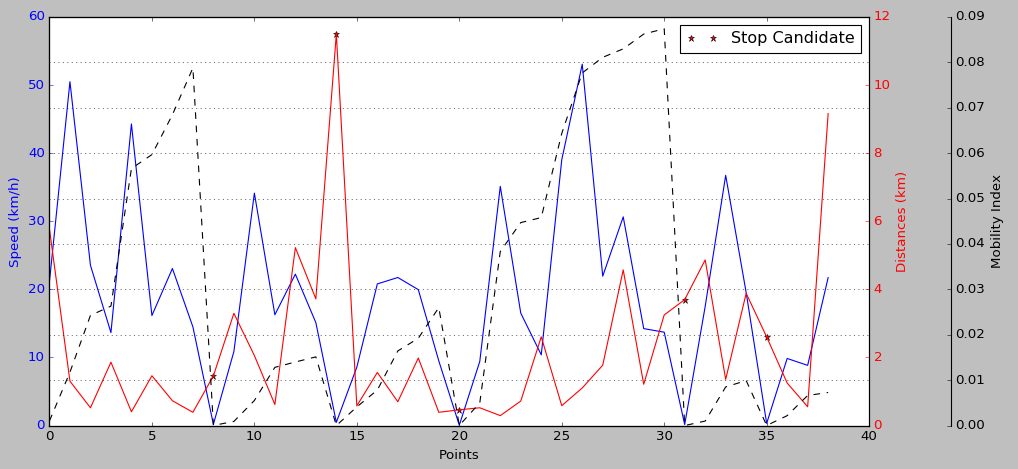
\includegraphics[width=0.95\textwidth]{images/reco_general.png}\\
	\caption{Result of identifying stop candidates for single user with their corresponding mobile index, distance and speed between the detected and previous point }
	\label{fig:reco_general}
\end{figure}

\FloatBarrier

\section{Clustering of Stops}

\FloatBarrier
\section{City Movements Graph}

\FloatBarrier